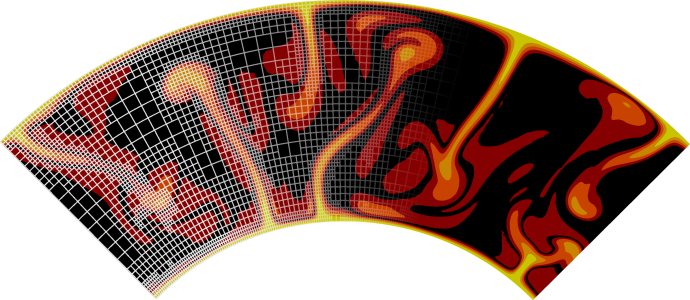
\includegraphics[height=1.25cm]{images/pictograms/aspect_logo}
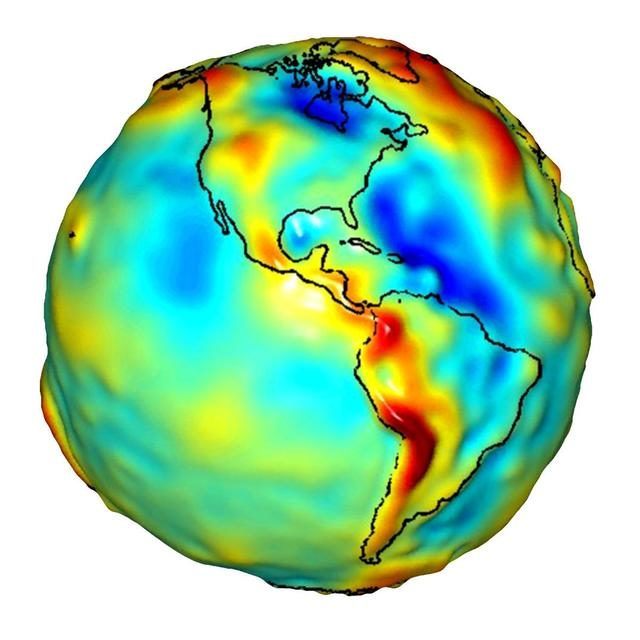
\includegraphics[height=1.25cm]{images/pictograms/gravity}

\includegraphics[height=1.25cm]{images/pictograms/benchmark}
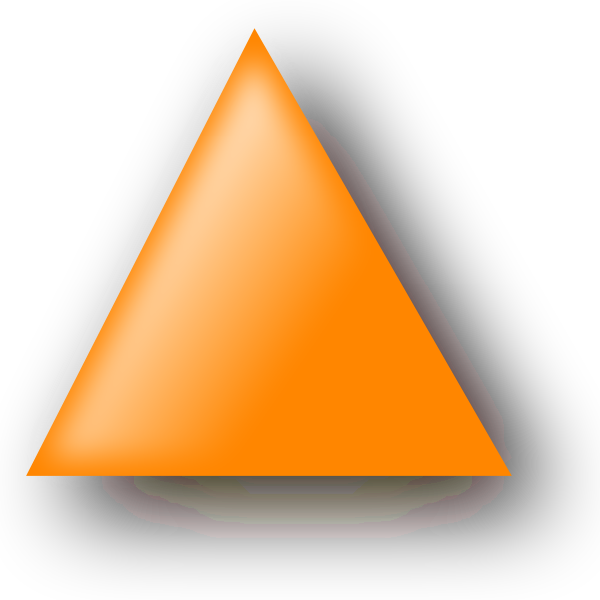
\includegraphics[height=1.25cm]{images/pictograms/triangle}
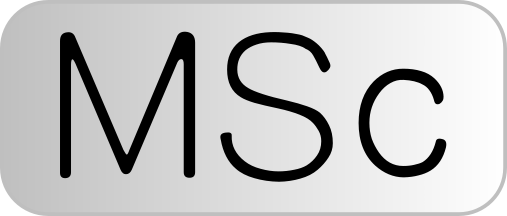
\includegraphics[height=1.25cm]{images/pictograms/msc}

\includegraphics[height=1.25cm]{images/pictograms/FEM}

\includegraphics[height=1.25cm]{images/pictograms/3d}

%%%%%%%%%%%%%%%%%%%%%%%%%%%%%%%%%%%%%%%%%%%%%%%%%%%%%%%%%%%%%%%%%%%%%%%%%%%%%%%%%%%%%%%%%%%%%%%%%%%

\begin{flushright} {\tiny {\color{gray} python\_codes/fieldstone\_96/text.tex}} \end{flushright}

\lstinputlisting[language=bash,basicstyle=\small]{python_codes/fieldstone_96/keywords.key}

\par\noindent\rule{\textwidth}{0.4pt}

\begin{center}
\fbox{\textbf{\huge \color{teal} P}}
Code at \url{https://github.com/cedrict/fieldstone/tree/master/python_codes/fieldstone_96}
\end{center}

\par\noindent\rule{\textwidth}{0.4pt}

{\sl This stone was developed in collaboration with Marjolein Blasweiler \& Bart Root}. 
\index{contributors}{B. Root} \index{contributors}{M. Blasweiler}

\par\noindent\rule{\textwidth}{0.4pt}

%%%%%%%%%%%%%%%%%%%%%%%%%%%%%%%%%%%%%%%%%%%%%%%%%%%%%%%%%%%%%%%%%%%%%%%%%%%%%%%%%%%%%%%%%%%%%%%%%%%

The domain is a half annulus and there are 6 materials in the domain: 
5 concentric layers and a 'blob', a half disc which center lies on the $z$-axis,  
as shown in the following figure.
\begin{center}
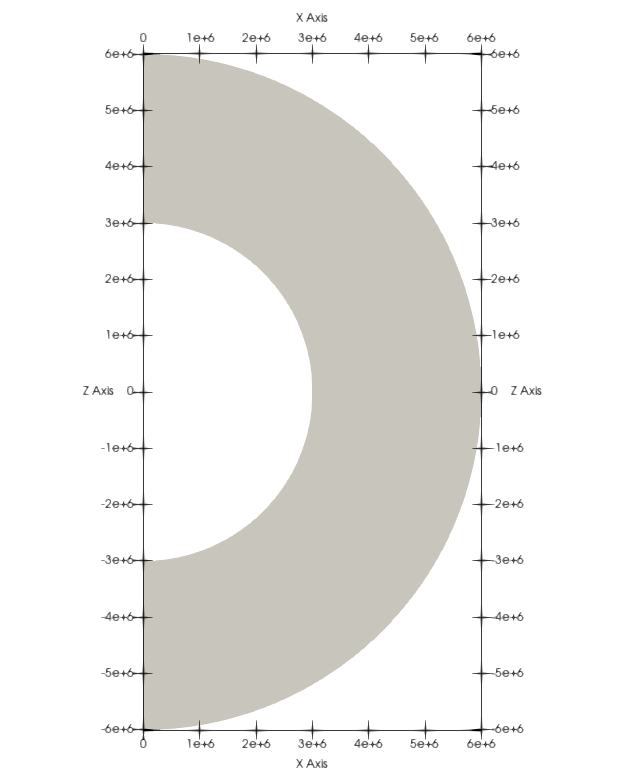
\includegraphics[width=5cm]{python_codes/fieldstone_96/images/domain}
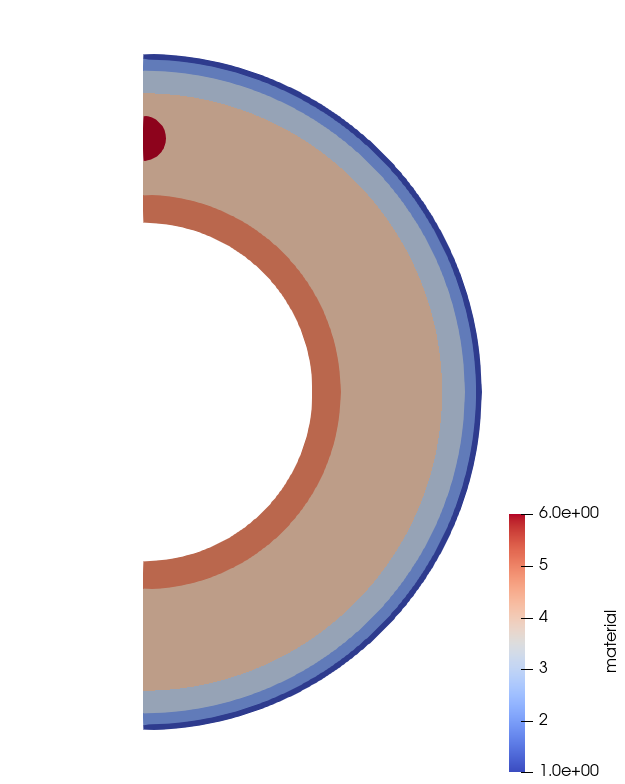
\includegraphics[width=5cm]{python_codes/fieldstone_96/images/domain2}\\
{\captionfont Example with $R_{inner}=3000~\si{\km}$ and $R_{outer}=6000~\si{\km}$.}
\end{center}
The thicknesses of the layers, their density, viscosity and the position, radius, density and viscosity 
of the blob can be adjusted. 

Gravity is radial and points towards the center of the planet. 
The code relies on $P_2\times P_1$ elements or Crouzeix-Raviart elements. 
Fluids are Newtoniani, incompressible and 
temperature effects are neglected. 
Boundary conditions are either free slip or no slip.

The code carries out four main tasks:
\begin{enumerate}
\item it solves the Stokes equations under the assumption that the problem is axisymmetric
\item from the obtained velocity and pressure fields, it computes strain rate and stress fields
\item it computes the dynamic topography on the inner and outer boundary
\item it computes the static gravity field as generated by the density field (again under the 
axisymmetric assumption)
\end{enumerate}
Results are then exported to ascii and vtu file(s).

The $r$ and $\theta$ spherical coordinates are defined as follows:
\begin{center}
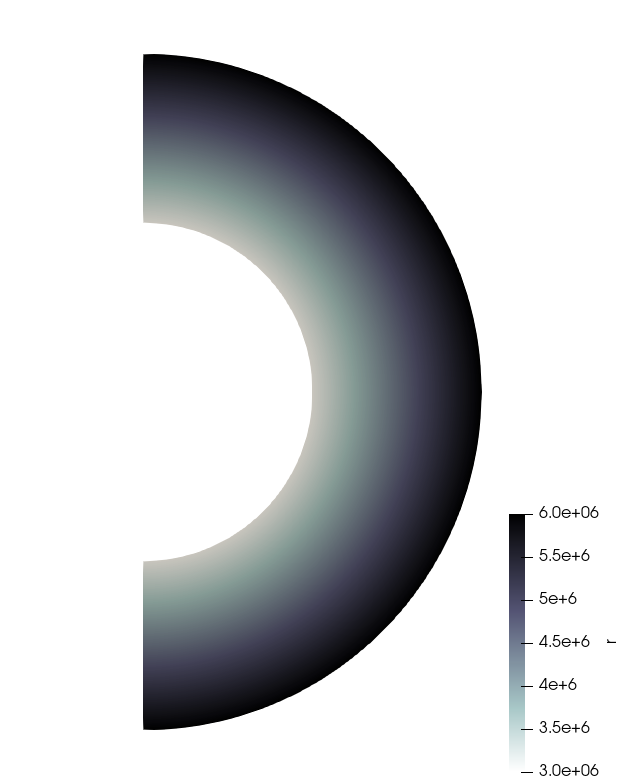
\includegraphics[width=5cm]{python_codes/fieldstone_96/images/radius}
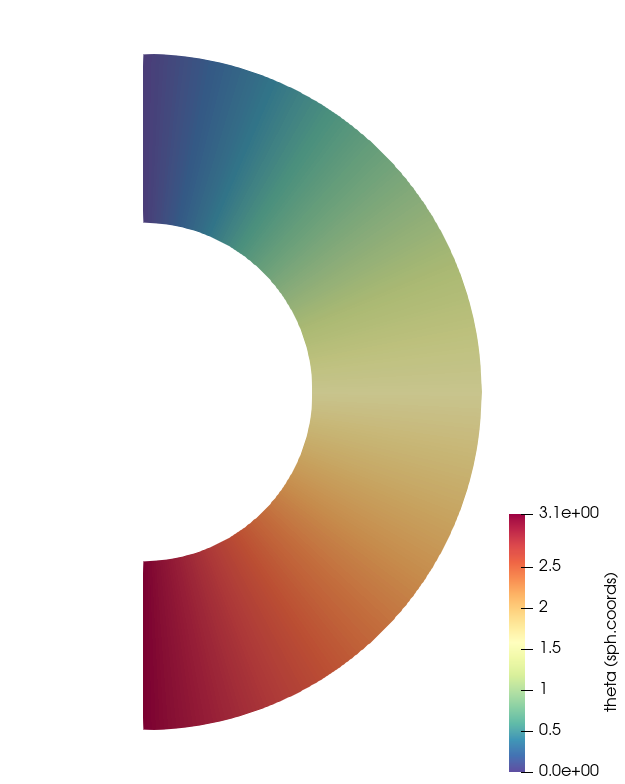
\includegraphics[width=5cm]{python_codes/fieldstone_96/images/theta}\\
{\captionfont Example with $R_{inner}=3000~\si{\km}$ and $R_{outer}=6000~\si{\km}$.}
\end{center}

%%%%%%%%%%%%%%%%%%%%%%%%%%%%%%%%%%%%%%%
\subsection*{How is mesh built}

The convex hull is built with points which are (on average) distant by $h$, 
a parameter specified by the user ({\tt hhh}).
The same is done for the material interfaces. 
The resulting set of nodes is then passed to the {\sl triangle} mesher, as explained 
in \stone~XXX.
This returns a mesh of triangles. However, we need mid-edge nodes for the Stokes equation
so this is what the {\tt mesh\_P1\_to\_P2} does. In the case of the Crouzeix-Raviart element, 
mid-triangle nodes are also added. 

\todo[inline]{include here figure with nodes}

The pressure solution $p$ is projected onto the velocity mesh and is then called $q$.



%%%%%%%%%%%%%%%%%%%%%%%%%%%%%%%%%%%%%%%
\subsection*{Axisymmetric considerations}

We here rely on axisymmetric cylindrical coordinates, see Section~\ref{MMM-ss:axicyleqs}.
As shown on the following figure we assume that the deformation/flow is independent of the angle 
$\theta$ so that the remaining space coordinates are $r$ and $z$.
\begin{center}
\input{tikz/tikz_axi}
\end{center}

Given the symmetry of the problem any term containing $\partial_\theta$ or $\upnu_\theta$ is zero.
The strain rate tensor given in Section~\ref{MMM-ss:srcc} then simplifies to:

\begin{eqnarray}
\dot\varepsilon_{rr} 
&=& \frac{\partial \upnu_r}{\partial r} \nn\\
\dot\varepsilon_{\theta\theta}  &=& \frac{\upnu_r}{r} \nn\\
\dot\varepsilon_{\theta r} = \dot\varepsilon_{r\theta}  &=& 0 \nn\\
\dot\varepsilon_{zz} &=& \frac{\partial \upnu_z}{\partial z} \nn\\
\dot{\varepsilon}_{rz} = \dot{\varepsilon}_{zr} 
&=& \frac{1}{2}\left( \frac{\partial \upnu_r}{\partial z} + \frac{\partial \upnu_z}{\partial r} \right) \nn\\
\dot{\varepsilon}_{\theta z} = \dot{\varepsilon}_{z \theta} &=& 0 \nn
\end{eqnarray}
Note that the term $\dot\varepsilon_{\theta\theta} $ is not zero!
The deviatoric stress tensor ${\bm \tau}=2\eta \dot{\bm \varepsilon}$ can be computed
as well as the full stress tensor ${\bm \sigma}=-p {\bm 1} + {\bm \tau}$. 


%%%%%%%%%%%%%%%%%%%%%%%%%%%%%%%%%%%%%%%%%%%
\subsection*{About pressure normalisation}

In spherical coordinates, we actually want to compute 
\[
\langle p \rangle _\Gamma = 
\frac{1}{4\pi R_o^2} \iiint \delta(r-R_o) p(\theta) r^2 \sin\theta \; dr d\theta d\phi 
= \frac{1}{2} \int_0^\pi p(\theta) \sin\theta \; d\theta
\]
The integral is then carried out by finding the elements for which 
two vertices are on the outside boundary, 
computing the angular opening $d\theta$, the average pressure 
along the edge and the value of $\sin\theta$ at the
middle of the edge. 
The obtained value is then subtracted from the pressure. 

%%%%%%%%%%%%%%%%%%%%%%%%%%%%%%%%%%%%%%%%%%%%%%%%%%%%%%%
\subsection*{From Cylindrical to Cartesian coordinates}

In cylindrical coordinates, and in the axisymmetric case
the strain rate tensor is given by
\[
\dot{\bm\varepsilon}(\vec\upnu)
=
\left(
\begin{array}{ccc}
\dot\varepsilon_{rr} & 0 & \dot{\varepsilon}_{rz} \\
0 & \dot{\varepsilon}_{\theta\theta}  & 0 \\
\dot{\varepsilon}_{zr} & 0 & \dot\varepsilon_{zz}
\end{array}
\right)
\]
We will now convert it to Cartesian coordinates using the equation 
from \url{https://www.brown.edu/Departments/Engineering/Courses/En221/Notes/Polar_Coords/Polar_Coords.htm}, where ${\bm T}$ is a tensor:
\[
{\bm T}_{\tiny Cyl}=
\left(
\begin{array}{ccc}
T_{rr}       & T_{r\theta}      & T_{rz} \\
T_{\theta r} & T_{\theta\theta} & T_{\theta z} \\
T_{z r}      & T_{z \theta}     & T_{zz}
\end{array}
\right)
=
\left(
\begin{array}{ccc}
 \cos \theta&\sin \theta&0 \\
-\sin \theta&\cos \theta&0 \\
0 & 0 & 1 
\end{array}
\right)
\cdot
\left(
\begin{array}{ccc}
T_{xx} & T_{xy} & T_{xz} \\
T_{yx} & T_{yy} & T_{yz} \\
T_{zx} & T_{zy} & T_{zz} 
\end{array}
\right)
\cdot
\left(
\begin{array}{ccc}
\cos \theta & -\sin \theta&0 \\
\sin \theta &  \cos \theta&0 \\
0 & 0 & 1 
\end{array}
\right)
\]

\[
{\bm T}_{\tiny Cart}=
\left(
\begin{array}{ccc}
T_{xx} & T_{xy} & T_{xz} \\
T_{yx} & T_{yy} & T_{yz} \\
T_{zx} & T_{zy} & T_{zz} 
\end{array}
\right)
=
\left(
\begin{array}{ccc}
 \cos \theta&-\sin \theta&0 \\
\sin \theta&\cos \theta&0 \\
0 & 0 & 1 
\end{array}
\right)
\cdot
\left(
\begin{array}{ccc}
T_{rr}       & T_{r\theta}      & T_{rz} \\
T_{\theta r} & T_{\theta\theta} & T_{\theta z} \\
T_{z r}      & T_{z \theta}     & T_{zz}
\end{array}
\right)
\cdot
\left(
\begin{array}{ccc}
\cos \theta & \sin \theta&0 \\
-\sin \theta &  \cos \theta&0 \\
0 & 0 & 1 
\end{array}
\right)
\]
In our case the calculation is taking place in the $(x,z)$
plane, i.e. $\theta=0$ so that the rotation matrices above 
are in fact identity matrices. 
We then simply have 
$\dot{\bm \varepsilon}_{\tiny Cart}=
\dot{\bm \varepsilon}_{\tiny Cyl}$.


%%%%%%%%%%%%%%%%%%%%%%%%%%%%%%%%%%%%%%%%%%%%%%%%%%%%%%%%%%%%%
\subsection*{From Cartesian to Spherical coordinates}

We have
\begin{eqnarray}
{\bm T}_{\tiny Sph}&=&
\left(
\begin{array}{ccc}
T_{rr}       & T_{r\theta}      & T_{r\phi} \\
T_{\theta r} & T_{\theta\theta} & T_{\theta\phi} \\
T_{\phi r}   & T_{\phi \theta}  & T_{\phi\phi}
\end{array}
\right) \nn\\
&=&
\left(
\begin{array}{ccc}
\sin\theta \cos\phi & \sin\theta \sin\phi & \cos\theta \\
\cos\theta \cos\phi & \cos\theta \sin\phi & -\sin\theta \\
-\sin\phi & \cos\phi & 0 
\end{array}
\right)
\cdot
\left(
\begin{array}{ccc}
T_{xx} & T_{xy} & T_{xz} \\
T_{yx} & T_{yy} & T_{yz} \\
T_{zx} & T_{zy} & T_{zz} 
\end{array}
\right)
\cdot
\left(
\begin{array}{ccc}
\sin\theta\cos\phi & \cos\theta\cos\phi & -\sin\phi \\
\sin\theta\sin\phi & \cos\theta\sin\phi & \cos\phi \\
\cos\theta & -\sin\theta & 0
\end{array}
\right) 
\nn\\
{\bm T}_{\tiny Cart} &=&
\left(
\begin{array}{ccc}
T_{xx} & T_{xy} & T_{xz} \\
T_{yx} & T_{yy} & T_{yz} \\
T_{zx} & T_{zy} & T_{zz} 
\end{array}
\right) \nn\\
&=&
\left(
\begin{array}{ccc}
\sin\theta\cos\phi & \cos\theta\cos\phi & -\sin\phi \\
\sin\theta\sin\phi & \cos\theta\sin\phi & \cos\phi \\
\cos\theta & -\sin\theta & 0
\end{array}
\right)
\cdot
\left(
\begin{array}{ccc}
T_{rr}       & T_{r\theta}      & T_{r\phi} \\
T_{\theta r} & T_{\theta\theta} & T_{\theta\phi} \\
T_{\phi r}   & T_{\phi \theta}  & T_{\phi\phi}
\end{array}
\right)
\cdot
\left(
\begin{array}{ccc}
\sin\theta \cos\phi & \sin\theta \sin\phi & \cos\theta \\
\cos\theta \cos\phi & \cos\theta \sin\phi & -\sin\theta \\
-\sin\phi & \cos\phi & 0 
\end{array}
\right)
\end{eqnarray}
In our case, calculations take place in the 
$(x,z)$-plane so we have $\phi=0$ and the equation above 
becomes
\[
\left(
\begin{array}{ccc}
T_{rr}       & T_{r\theta}      & T_{r\phi} \\
T_{\theta r} & T_{\theta\theta} & T_{\theta\phi} \\
T_{\phi r}   & T_{\phi \theta}  & T_{\phi\phi}
\end{array}
\right)
=
\left(
\begin{array}{ccc}
\sin\theta  & 0 & \cos\theta \\
\cos\theta  & 0 & -\sin\theta \\
0 & 1 & 0 
\end{array}
\right)
\cdot
\left(
\begin{array}{ccc}
T_{xx} & T_{xy} & T_{xz} \\
T_{yx} & T_{yy} & T_{yz} \\
T_{zx} & T_{zy} & T_{zz} 
\end{array}
\right)
\cdot
\left(
\begin{array}{ccc}
\sin\theta & \cos\theta & 0 \\
0 & 0 & 1 \\
\cos\theta & -\sin\theta & 0
\end{array}
\right)
\]
We define $c_\theta=\cos\theta$, $s_\theta=\sin\theta$ so that
\[
\left(
\begin{array}{ccc}
T_{rr}       & T_{r\theta}      & T_{r\phi} \\
T_{\theta r} & T_{\theta\theta} & T_{\theta\phi} \\
T_{\phi r}   & T_{\phi \theta}  & T_{\phi\phi}
\end{array}
\right)
=
\left(
\begin{array}{ccc}
s_\theta  & 0 & c_\theta \\
c_\theta  & 0 & -s_\theta \\
0 & 1 & 0 
\end{array}
\right)
\cdot
\left(
\begin{array}{ccc}
T_{xx} & T_{xy} & T_{xz} \\
T_{yx} & T_{yy} & T_{yz} \\
T_{zx} & T_{zy} & T_{zz} 
\end{array}
\right)
\cdot
\left(
\begin{array}{ccc}
s_\theta & c_\theta & 0 \\
0 & 0 & 1 \\
c_\theta & -s_\theta & 0
\end{array}
\right)
\]
As we have seen above we have 
\[
\dot{\bm\varepsilon}_{\tiny Cart}
=
\left(
\begin{array}{ccc}
\dot\varepsilon_{xx} & 0 & \dot{\varepsilon}_{xz} \\
0 & \dot{\varepsilon}_{yy}  & 0 \\
\dot{\varepsilon}_{xz} & 0 & \dot\varepsilon_{zz}
\end{array}
\right)
\]
so 
\begin{eqnarray}
\dot{\bm \varepsilon}_{\tiny Sph}=
\left(
\begin{array}{ccc}
\dot\varepsilon_{rr}       & \dot\varepsilon_{r\theta}      & \dot\varepsilon_{r\phi} \\
\dot\varepsilon_{\theta r} & \dot\varepsilon_{\theta\theta} & \dot\varepsilon_{\theta\phi} \\
\dot\varepsilon_{\phi r}   & \dot\varepsilon_{\phi \theta}  & \dot\varepsilon_{\phi\phi}
\end{array}
\right)
&=&
\left(
\begin{array}{ccc}
s_\theta  & 0 & c_\theta \\
c_\theta  & 0 & -s_\theta \\
0 & 1 & 0 
\end{array}
\right)
\cdot
\left(
\begin{array}{ccc}
\dot\varepsilon_{xx} & 0 & \dot{\varepsilon}_{xz} \\
0 & \dot{\varepsilon}_{yy}  & 0 \\
\dot{\varepsilon}_{xz} & 0 & \dot\varepsilon_{zz}
\end{array}
\right)
\cdot
\left(
\begin{array}{ccc}
s_\theta & c_\theta & 0 \\
0 & 0 & 1 \\
c_\theta & -s_\theta & 0
\end{array}
\right)  \nonumber\\
&=&
\left(
\begin{array}{ccc}
s_\theta  & 0 & c_\theta \\
c_\theta  & 0 & -s_\theta \\
0 & 1 & 0 
\end{array}
\right)
\cdot
\left(
\begin{array}{ccc}
\dot\varepsilon_{xx} s_\theta + 
\dot\varepsilon_{xz} c_\theta  & 
\dot\varepsilon_{xx} c_\theta - 
\dot\varepsilon_{xz} s_\theta  &
0 \\
0 & 0 & \dot{\varepsilon}_{yy}  
\\
\dot\varepsilon_{xz} s_\theta + 
\dot\varepsilon_{zz} c_\theta  &
\dot\varepsilon_{xz} c_\theta - 
\dot\varepsilon_{zz} s_\theta  &
0 
\end{array}
\right)  \nonumber\\
&=&
\left(
\begin{array}{ccc}
\dot\varepsilon_{xx} s_\theta^2 + 
2 \dot\varepsilon_{xz} c_\theta  s_\theta +
\dot\varepsilon_{zz} c_\theta ^2  
& 
\dot\varepsilon_{xx} c_\theta s_\theta - 
\dot\varepsilon_{xz} s_\theta^2  +
\dot\varepsilon_{xz} c_\theta^2 - 
\dot\varepsilon_{zz} s_\theta c_\theta 
& 0 \\ \\
\dot\varepsilon_{xx} s_\theta c_\theta+ 
\dot\varepsilon_{xz} c_\theta^2  -
\dot\varepsilon_{xz} s_\theta^2 -
\dot\varepsilon_{zz} c_\theta s_\theta 
&
\dot\varepsilon_{xx} c_\theta^2 - 
2\dot\varepsilon_{xz} s_\theta c_\theta +
\dot\varepsilon_{zz} s_\theta^2  
& 0 
\\ \\
0 & 0 & \dot{\varepsilon}_{yy} 
\end{array}
\right)  \nonumber
\end{eqnarray}
We can easily verify that the trace of this tensor is zero.

The deviatoric stress is given by 
${\bm \tau}=2\eta \dot{\bm \varepsilon}$,
the traction at the surface  by 
$\vec{t}={\bm \tau}\cdot \vec{n}$ (
with $\vec{n}=\vec{e}_r$ at the surface in Spherical coordinates) and the normal to the surface component of this traction 
is given by
\[
t_r = \vec{t}\cdot \vec{n} = ({\bm \tau}\cdot \vec{n})\cdot \vec{n} = \tau_{rr}
\]


%_____________________________________________________________
\subsection*{A proxy for elasto-viscous lithospheric rheology}

The implementation of elastic behaviour in a velocity-pressure code is not trivial 
and is presented in Section~\ref{MMM-ss:evrheo}.
In the end the lithospheric viscosity will be an effective viscosity given by
\[
\eta_{eff} = \frac{\mu \delta t}{1+\mu/\eta \delta t} 
\]
This is only used if \texttt{use\_ev} is true.

%__________________________________________________________________________
\subsection*{Computing the total mass of the planet based on radial profiles}

REMARK: for now the code does not use radial profiles.


The mass of the shell is given by
\[
M= \iiint_\Omega \rho(r) r^2 \sin\theta dr d\theta d\phi
= 4\pi \int_{Ri}^{Ro} \rho(r) r^2 dr
\]
The density profile is known on N intervals ($N+1$ points) between $Ri$ and $Ro$ so that 
\[
M = 4\pi \sum_{i=1}^N \int_{r_i^-}^{r_i^+} \rho(r) r^2 dr
\]
where $r_i^-$ and $r_i^+$ are the bounds of the interval $i$
under consideration.
Over this interval the density is linear and goes from $\rho(r_i^-)=\rho_i^-$ to $\rho(r_i^+)=\rho_i^+$. 
We have then $\rho(r)=ar+b$ with 
\[
\rho(r) = \frac{\rho_i^+-\rho_i^-}{r_i^+-r_i^-}(r-r_i^-)+\rho_i^-
\qquad\quad
a= \frac{\rho_i^+-\rho_i^-}{r_i^+-r_i^-}
\qquad\quad
b=-\frac{\rho_i^+-\rho_i^-}{r_i^+-r_i^-}r_i^- + \rho_i^-
\]
so that the mass of a shell corresponding to interval $i$ 
bounded by $r_i^-$ and $r_i^+$ is
\begin{eqnarray}
M_i 
&=& \int_{r_i^-}^{r_i^+} (ar+b)r^2 dr  \nonumber\\
&=& \int_{r_i^-}^{r_i^+} (ar^3+br^2) dr  \nonumber\\
&=& a\int_{r_i^-}^{r_i^+} r^3 dr 
+b\int_{r_i^-}^{r_i^+} r^2 dr \nonumber\\
&=& \frac{a}{4} \left[ (r_i^+)^4 -(r_i^-)^4  \right]
+\frac{b}{3} \left[ (r_i^+)^3 -(r_i^-)^3 \right]
\end{eqnarray}
We can now look at each provided density profile for the planet and
compute the corresponding mass.


%--------------------------------------------------
\subsection*{Elliptic blob}

The eccentricity $e$ of an ellipse is defined as 
\[
e=\sqrt{1-\frac{b^2}{a^2}}
\]
where $a$ is the length of the semi-major axis and $b$ is the length of the semi-minor axis.

The eccentricity of ellipse is less than 1. The eccentricity of a ellipse helps us to understand how circular it is with reference to a circle. Eccentricity also measures the ovalness of the ellipse and eccentricity close to one refers to high degree of ovalness.

In our case we assume that the semi-major axis is along the $x$-axis.
We will set $b=R_{blob}$ and vary the eccentricity so as to obtain a circle ($e=1$) or an ellipse $e<1$.
We have
\[
e^2 = 1 -\frac{b^2}{a^2}
\quad
\rightarrow
\quad
1-e^2 = \frac{b^2}{a^2}
\quad
\rightarrow
\quad
\frac{1}{1-e^2} = \frac{a^2}{b^2}
\quad
\rightarrow
\quad
a^2 = b^2 \frac{1}{1-e^2} 
\quad
\rightarrow
\quad
a = b \sqrt{\frac{1}{1-e^2}}
\]

The volume of the blob is then 
\[
V_{blob} = \frac{4\pi}{3}a^2b
\]


 
%--------------------------------------------------
\subsection*{Gravity calculations}

This is an axisymmetric problem so the mesh is generated for a single 
value of the cylindrical coordinates $\theta$ angle. 
This makes gravity calculations a bit more difficult because each triangle 
of the mesh corresponds in 3D to a ring of matter with this triangular cross section. 
I have therefore chosen to divide this ring in {\tt nel\_phi} segments. 
Each segment has a given volume and therefore mass, 
and having computed its center its generated gravity field can be added. 
The volume of such a block is 
$\iiint_{block} r dr d\theta dz =\iint_\triangle rdrdz \cdot \int d\theta$.  
The first integral is carried out for each triangle and the result is stored 
in the {\tt arear} array. 


Look at Morgan (1965) \cite{morg65} for gravity anomalies above sinking sphere. 

Open question: what is an optimal value for {\tt nel\_phi} ?








%%%%%%%%%%%%%%%%%%%%%%%%%%%%%%%%%%%%%%%%%%%%%%%%%%%%%%%%%%%%%%%%%%%%%%%%%%%%%%%%%%%%%%%%%%%%%%%%%%%
\section*{Benchmarking}

The type of model that this \stone is designed to simulate does not admit an 
analytical mechanical solution, so we will need to compare our results with those 
of an other code, typically \aspect. 
However, two simple benchmarks can be run for the gravity calculations: 
a hollow sphere of constant density, and a full sphere (only the blob has non zero density).




\newpage
%%%%%%%%%%%%%%%%%%%%%%%%%%%%%%%%%%%%%%
\subsection*{Stokes benchmark - test0}

The planet has an inner radius of 3000km and an outer radius of 6000km.
The material interfaces are placed at $R=5900~\si{\km}$, $R=5700~\si{\km}$, $R=5300~\si{\km}$, $R=3500~\si{\km}$.
To start with we assign a zero density to all layers and a density of -10 to the blob. 
All layers have a viscosity of 1e21 while the blob has a viscosity of 1e25.
Dynamic topography cannot be computed because density is zero at the surface.
Free slip at top and bottom, hhh=200.

\begin{center}
\includegraphics[width=8cm]{python_codes/fieldstone_96/results/stokes_test0/surface_vt}
\includegraphics[width=8cm]{python_codes/fieldstone_96/results/stokes_test0/cmb_vt}\\
\includegraphics[width=8cm]{python_codes/fieldstone_96/results/stokes_test0/surface_p}
\includegraphics[width=8cm]{python_codes/fieldstone_96/results/stokes_test0/cmb_p}\\
\includegraphics[width=8cm]{python_codes/fieldstone_96/results/stokes_test0/surface_q}
\includegraphics[width=8cm]{python_codes/fieldstone_96/results/stokes_test0/cmb_q}\\
{\captionfont Tangential velocity and pressure at surface and cmb for both finite element pairs.}
\end{center}

\todo[inline]{do with aspect and plot against my data}

\begin{center}
\includegraphics[width=5cm]{python_codes/fieldstone_96/results/stokes_test0/vel}
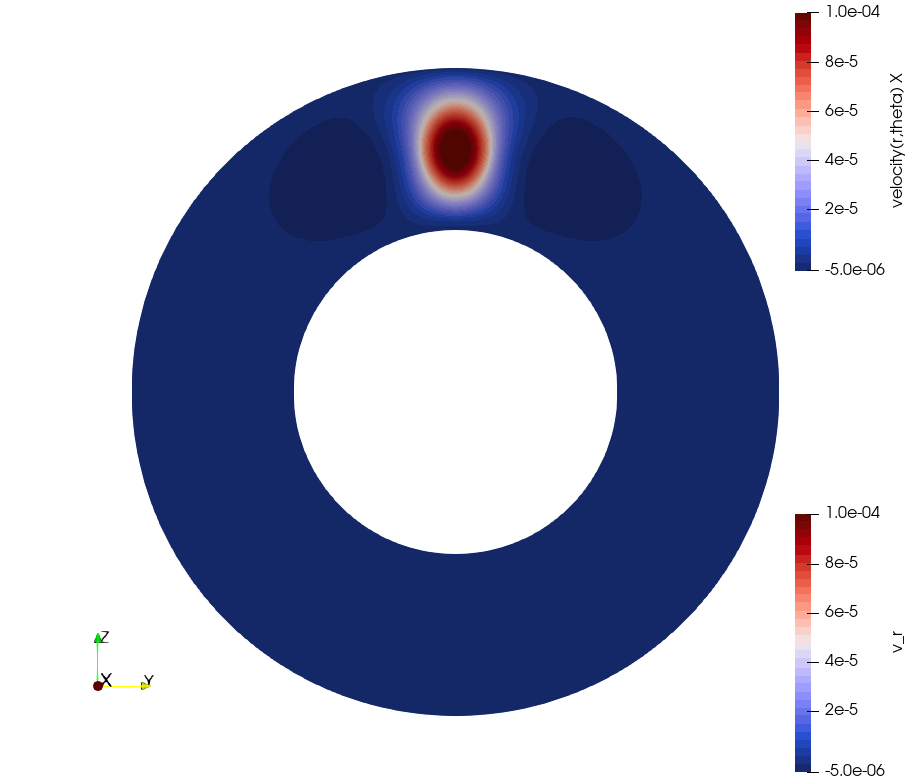
\includegraphics[width=5cm]{python_codes/fieldstone_96/results/stokes_test0/vr}
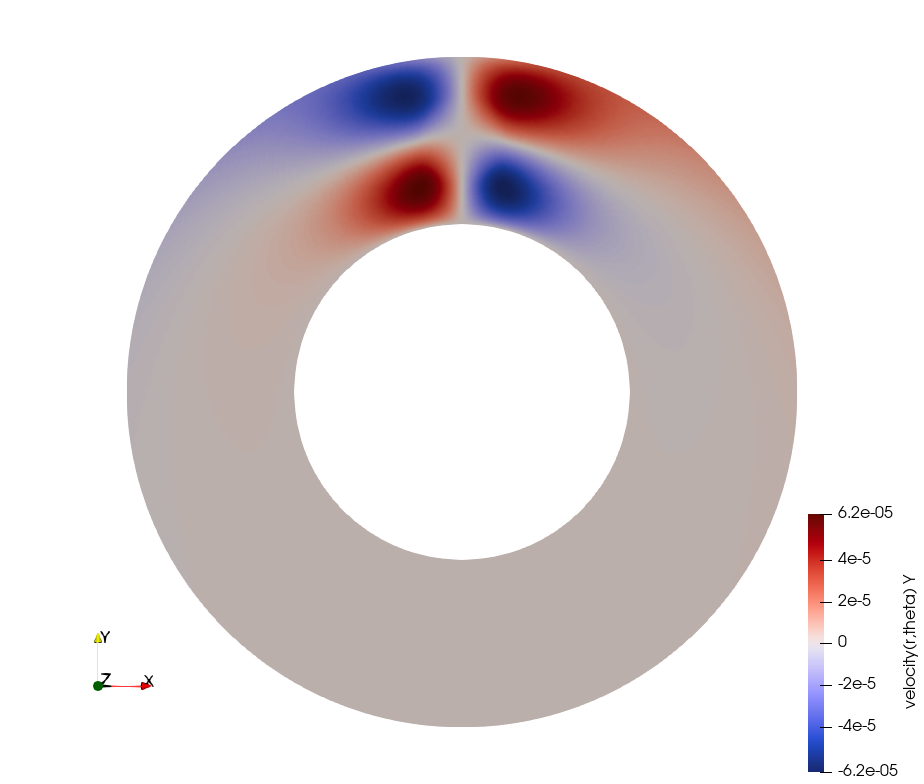
\includegraphics[width=5cm]{python_codes/fieldstone_96/results/stokes_test0/vt}\\
\includegraphics[width=5cm]{python_codes/fieldstone_96/results/stokes_test0/rho}
\includegraphics[width=5cm]{python_codes/fieldstone_96/results/stokes_test0/press}
\end{center}


\newpage
%%%%%%%%%%%%%%%%%%%%%%%%%%%%%%%%%%%%%%
\subsection*{Stokes benchmark - test1}

This is an identical setup to test0, but now all layers have a density of 3000 and the blob a density of 2990.
The velocity solution should be identical but the pressure should now showcase the hydrostatic signal too.

\begin{center}
\includegraphics[width=8.5cm]{python_codes/fieldstone_96/results/stokes_test1/surface_vt_cr}
\includegraphics[width=8.5cm]{python_codes/fieldstone_96/results/stokes_test1/surface_vt_p2p1}\\
\includegraphics[width=8.5cm]{python_codes/fieldstone_96/results/stokes_test1/surface_p_cr}
\includegraphics[width=8.5cm]{python_codes/fieldstone_96/results/stokes_test1/surface_p_p2p1}\\
\includegraphics[width=8.5cm]{python_codes/fieldstone_96/results/stokes_test1/surface_q_cr}
\includegraphics[width=8.5cm]{python_codes/fieldstone_96/results/stokes_test1/surface_q_p2p1}\\
\includegraphics[width=8.5cm]{python_codes/fieldstone_96/results/stokes_test1/surface_taurr_cr}
\includegraphics[width=8.5cm]{python_codes/fieldstone_96/results/stokes_test1/surface_taurr_p2p1}\\
\includegraphics[width=8.5cm]{python_codes/fieldstone_96/results/stokes_test1/surface_dynamic_topography_cr.pdf}
\includegraphics[width=8.5cm]{python_codes/fieldstone_96/results/stokes_test1/surface_dynamic_topography_p2p1.pdf}\\
{\captionfont Tangential velocity and pressure at surface for both finite element pairs.}
\end{center}

-------

\begin{center}
\includegraphics[width=8.5cm]{python_codes/fieldstone_96/results/stokes_test1/cmb_vt_cr}
\includegraphics[width=8.5cm]{python_codes/fieldstone_96/results/stokes_test1/cmb_vt_p2p1}\\
\includegraphics[width=8.5cm]{python_codes/fieldstone_96/results/stokes_test1/cmb_p_cr}
\includegraphics[width=8.5cm]{python_codes/fieldstone_96/results/stokes_test1/cmb_p_p2p1}\\
\includegraphics[width=8.5cm]{python_codes/fieldstone_96/results/stokes_test1/cmb_q_cr}
\includegraphics[width=8.5cm]{python_codes/fieldstone_96/results/stokes_test1/cmb_q_p2p1}\\
\includegraphics[width=8.5cm]{python_codes/fieldstone_96/results/stokes_test1/cmb_taurr_cr}
\includegraphics[width=8.5cm]{python_codes/fieldstone_96/results/stokes_test1/cmb_taurr_p2p1}\\
\includegraphics[width=8.5cm]{python_codes/fieldstone_96/results/stokes_test1/cmb_dynamic_topography_cr.pdf}
\includegraphics[width=8.5cm]{python_codes/fieldstone_96/results/stokes_test1/cmb_dynamic_topography_p2p1.pdf}\\
{\captionfont Tangential velocity and pressure at cmb for both finite element pairs.}
\end{center}

We see that the velocity field is actually showcasing a lot of random variations
which can only be attributed to using the full density... WHY ? 


\begin{center}
\includegraphics[width=5cm]{python_codes/fieldstone_96/results/stokes_test1/vel}
\includegraphics[width=5cm]{python_codes/fieldstone_96/results/stokes_test1/press}
\end{center}






\newpage
%%%%%%%%%%%%%%%%%%%%%%%%%%%%%%%%%%%%%%
\subsection*{Stokes benchmark - test2}


with $\rho_1=2900$,  $\rho_2=3000$,  $\rho_3=3300$, $\rho_4=4000$,  $\rho_5=4500$ and 
with $\eta_1=1e23$,  $\eta_2=1e21$,  $\eta_3=5e21$, $\eta_4=5e20$, $\eta_4=1e20$.
The blob is situated 1000km below the surface, and it has a radius of 400km and density of 3100kg/m3 and viscosity $10^{25}$.
Gravity is set to 10 for simplicity.

{\tt script\_test1}

\begin{center}
\includegraphics[width=5cm]{python_codes/fieldstone_96/results/stokes_test2/materials}
\includegraphics[width=5cm]{python_codes/fieldstone_96/results/stokes_test2/rho}
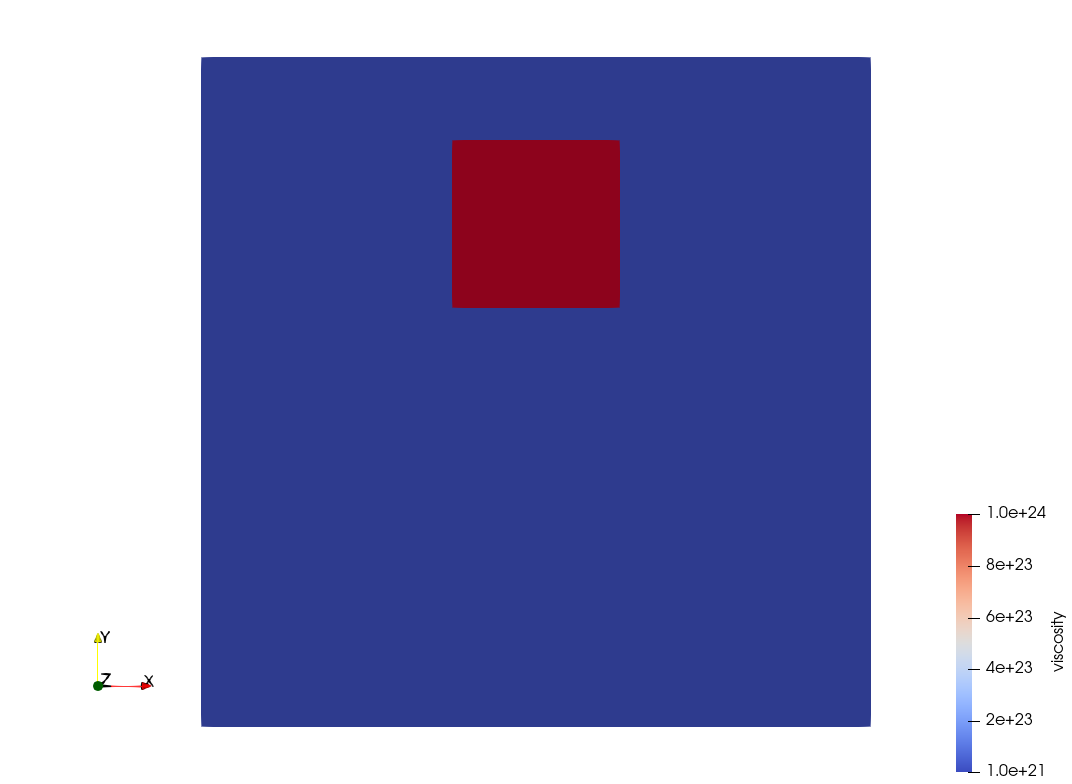
\includegraphics[width=5cm]{python_codes/fieldstone_96/results/stokes_test2/eta}
\end{center}


\begin{center}
\includegraphics[width=5cm]{python_codes/fieldstone_96/results/stokes_test2/vel}
\includegraphics[width=5cm]{python_codes/fieldstone_96/results/stokes_test2/press}
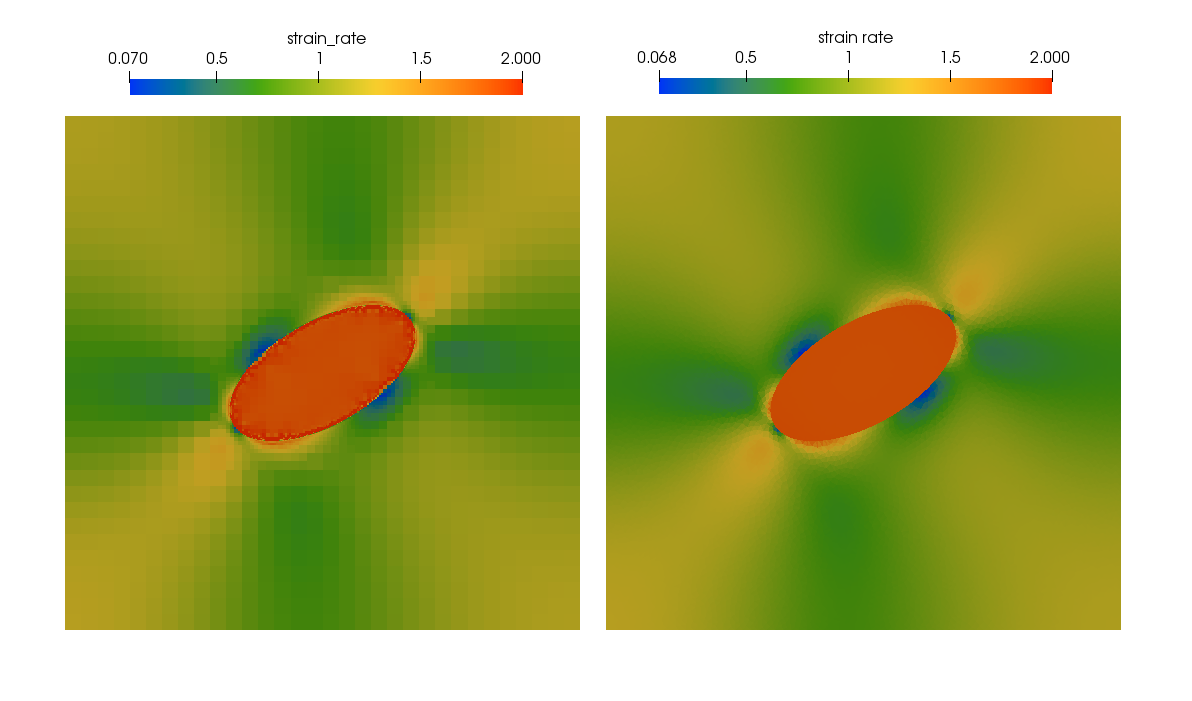
\includegraphics[width=5cm]{python_codes/fieldstone_96/results/stokes_test2/sr}
\end{center}



\begin{center}
\includegraphics[width=8cm]{python_codes/fieldstone_96/results/stokes_test2/surface_vt}
\includegraphics[width=8cm]{python_codes/fieldstone_96/results/stokes_test2/cmb_vt}\\
\includegraphics[width=8cm]{python_codes/fieldstone_96/results/stokes_test2/dynamic_topography_cmb}
\includegraphics[width=8cm]{python_codes/fieldstone_96/results/stokes_test2/dynamic_topography_surf}\\
\end{center}





\newpage
%%%%%%%%%%%%%%%%%%%%%%%%%%%%%%%%%%%%%%%%%%%%%%%%%%
\subsection*{gravity benchmark \#1: hollow sphere}

The planet has an inner radius of 3000km and an outer radius of 6000km.
All 5 layers and blob have the same density of 3000kg/m3.
Gravity is computed at a height of 10km above the surface.

{\tt script\_hollow\_sphere}

\begin{center}
\includegraphics[width=5cm]{python_codes/fieldstone_96/results/gravity_hollow_sphere/rho}
\end{center}

\begin{center}
\includegraphics[width=8cm]{python_codes/fieldstone_96/results/gravity_hollow_sphere/grav.pdf}
\end{center}

\newpage
%%%%%%%%%%%%%%%%%%%%%%%%%%%%%%%%%%%%%%%%%%%%%%
\subsection*{gravity benchmark \#2: only blob}

The planet has an inner radius of 3000km and an outer radius of 6000km,
although it does not matter since all 5 layers have a zero density. 
The blob is situated 1000km below the surface, and it has a radius of 400km and density of 200kg/m3.
Gravity is computed at a height of 10km above the surface.

{\tt script\_only\_blob}

\begin{center}
\includegraphics[width=5cm]{python_codes/fieldstone_96/results/gravity_only_blob/rho}
\end{center}

\begin{center}
\includegraphics[width=8cm]{python_codes/fieldstone_96/results/gravity_only_blob/grav.pdf}
\end{center}













\newpage
%%%%%%%%%%%%%%%%%%%%%%%%%%%%%%%%%%%%%%%%%%%%
\section*{Basic facts about the planet Mars}

Facts about planet Mars\footnote{\url{https://en.wikipedia.org/wiki/Mars}}:
\begin{itemize}
\item average radius $R=3389.5 \pm 0.2 \si{\km}$
\item equatorial radius $3396.2 \pm 0.1 \si{\km}$
\item polar radius $3376.2 \pm 0.1 \si{\km}$
\item volume $1.6318 \cdot 10^{20} \si{\cubic\metre}$
\item mass $6.4171 \cdot 10^{23}\si{\kilo\gram}$
\item mean density $\langle\rho\rangle= 3934\si{\kilo\gram\per\cubic\meter}$
\item moment of inertia $I=0.3644 \pm 0.0005$
\item surface gravity $g=3.72076 \si{\metre\per\square\second}$
\end{itemize}

The surface gravity can be obtained with 
\[
g_{surf}=\frac{{\cal G} M}{R^2} 
=\frac{6.67430 \cdot 10^{-11} \; 6.4171 \cdot 10^{23} }{(3.3895\cdot 10^6)^2}
\simeq 3.727977
\]

%%%%%%%%%%%%%%%%%%%%%%%%%%%%%%%%%%%%%%%%%%%%%%%%
\section*{Internal structure of the planet Mars}

The internal structure of the planet is not settled although 
it is now widely accepted that the planet has a core. News alert: \cite{khcv21,stkb21,knpb21}. 

B. Steinberger was kind enough to communicate to us the density and viscosity 
profiles used in Steinberger \etal (2010) \cite{stwt10} \footnote{Files sent to us 
we slightly altered for the purpose of this work. The density profile was missing 
the 50km near the center of the planet so padding was used. The viscosity profile 
starts below the moho at 50\si{\km} and stopped at the cmb.}:

\begin{center}
\includegraphics[width=5.7cm]{python_codes/fieldstone_96/data/rho_steinberger}
\includegraphics[width=5.7cm]{python_codes/fieldstone_96/data/rho_samuelA}
\includegraphics[width=5.7cm]{python_codes/fieldstone_96/data/rho_samuelB}\\
\includegraphics[width=5.7cm]{python_codes/fieldstone_96/data/eta_steinberger}
\includegraphics[width=5.7cm]{python_codes/fieldstone_96/data/eta_samuelA}
\includegraphics[width=5.7cm]{python_codes/fieldstone_96/data/eta_samuelB}\\
{\captionfont Data curtesy of B. Steinberger, from \cite{stwt10}.
Samuel data via private communication.} \\
{\tiny {\color{gray} in python\_codes/fieldstone\_96/data/}}
\end{center}

\begin{center}
\includegraphics[width=5.7cm]{python_codes/fieldstone_96/images/stwt10_b}
\includegraphics[width=5.7cm]{python_codes/fieldstone_96/images/stwt10_c}
\includegraphics[width=5.7cm]{python_codes/fieldstone_96/images/stwt10_d}\\
{\captionfont Taken from Steinberger \etal (2010) \cite{stwt10}}
\end{center}

In table 1 of Steinberger \etal \cite{stwt10}: crust thickness is set to 50km. The core radius is set 
to 1389.5km. However in the data set we were sent it seems that the cmb is at 1422\si{\km}
radius.
To simplify things we take $R=3389\si{\km}$ and $R_{cmb}=1422\si{\km}$ in the code.
\todo[inline]{Sort this out}






